%%---------------------------------------------------------------------------%%
%% Beamer ORNL Presentation Template
%%---------------------------------------------------------------------------%%

\documentclass{beamer}
%% The amssymb package provides various useful mathematical symbols
\usepackage{amssymb}
%% The amsthm package provides extended theorem environments
\usepackage{amsthm} \usepackage{amsmath} \usepackage{tmadd,tmath}
\usepackage{booktabs}
\usepackage{multirow}
\usepackage{subfigure}
\usepackage[compatibility=false]{caption}
\usepackage{tikz}
\usepackage{ragged2e}
\usepackage{algorithm,algorithmic}

\usetikzlibrary{arrows}

%%---------------------------------------------------------------------------%%
%% THEME SETUP

\usetheme{CambridgeUS}
\usecolortheme{spruce}

%%---------------------------------------------------------------------------%%
%% SETUP STUFF
%%---------------------------------------------------------------------------%%

\logo{
\includegraphics[width=2cm]{new_logo}}

\setbeamercolor{item}{fg=MSUgreen}
\beamertemplatenavigationsymbolsempty
\setbeamertemplate{headline}{}
\setbeamertemplate{footline}{
  \insertframenumber/\inserttotalframenumber}
\setbeamertemplate{title page}
{
  \begin{tabular}{cr}
    \begin{minipage}{5.5cm}
      {\RaggedRight \bf \large \textcolor{MSUgreen}{\inserttitle}}\\
      \vspace{\baselineskip}\\
      \insertauthor\\
      \vspace{0.5\baselineskip}\\
      \insertinstitute\\
      \insertdate
    \end{minipage}
  \end{tabular}
}

\newlength{\DUtablewidth} % internal use in tables

%%---------------------------------------------------------------------------%%
%% TITLE

\title[MCREX]{Using Monte Carlo Algorithms to Achieve Resiliency \& Performance
  at Scale for Linear and Nonlinear Solver Applications}
\author{Thomas Evans \and Steven Hamilton}
\date[DOE, 2016]{DOE RX-Solvers \\ January 29, 2016}
\institute[ORNL]{Oak Ridge National Lab}

%%---------------------------------------------------------------------------%%
\begin{document}
%%---------------------------------------------------------------------------%%

{
  \usebackgroundtemplate{
    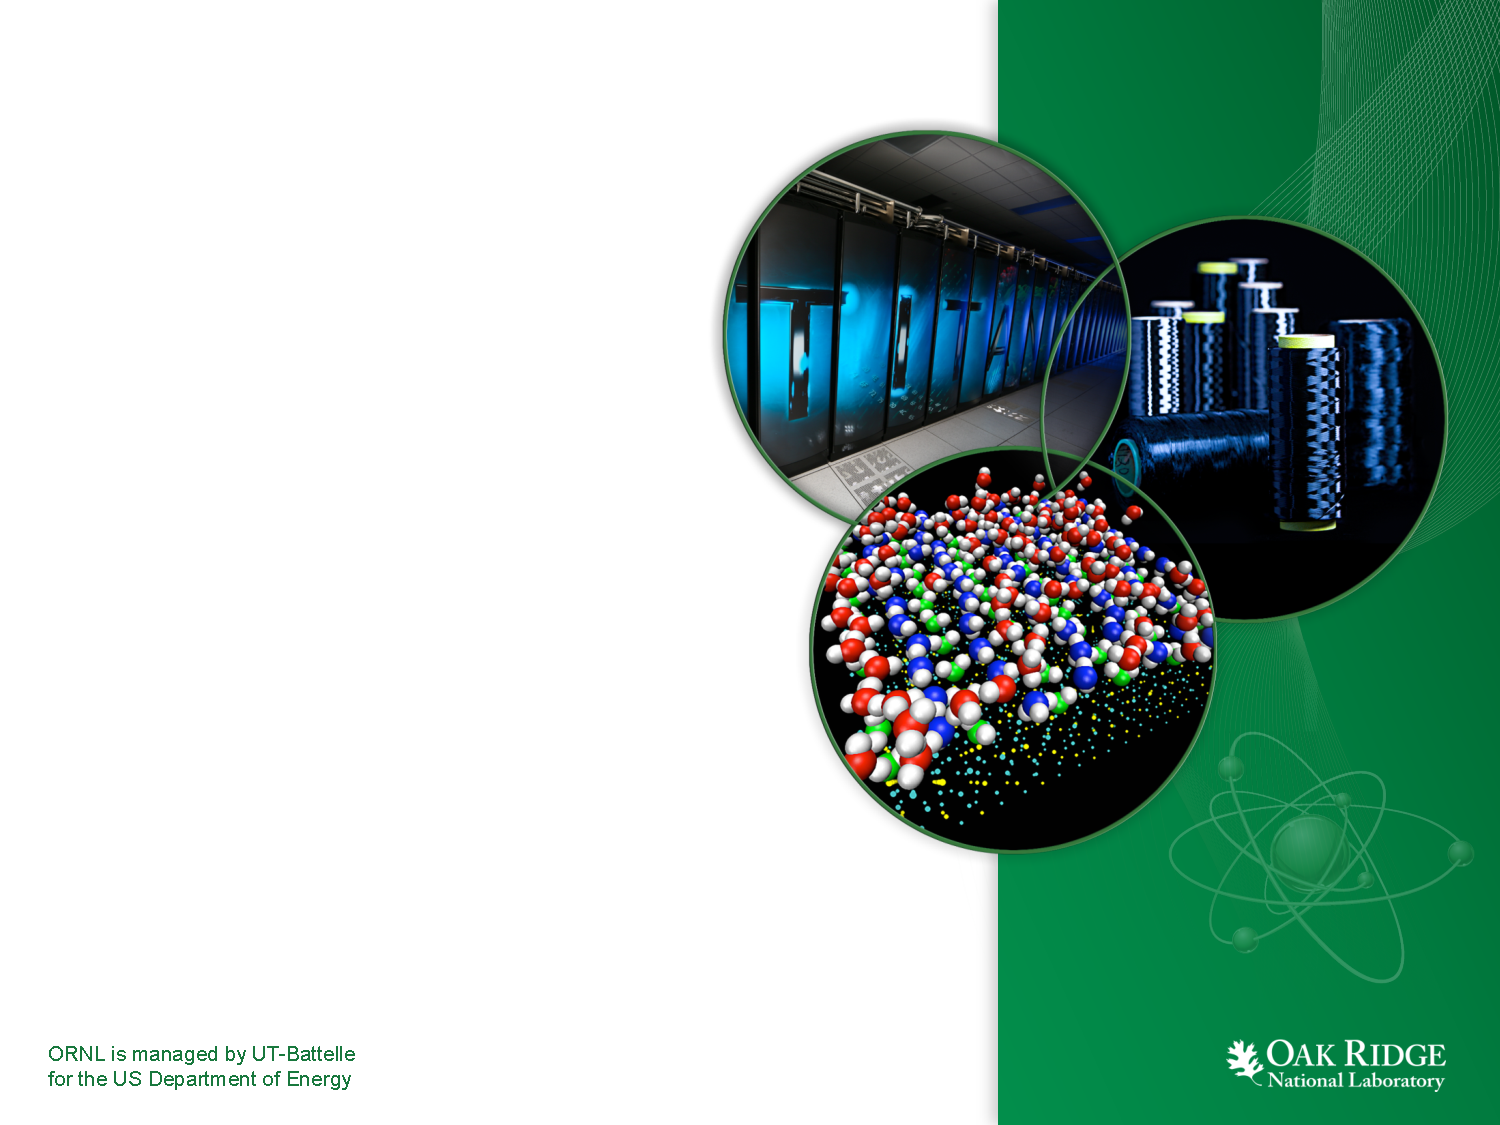
\includegraphics[width=\paperwidth,height=\paperheight]{title_template}}
  \setbeamertemplate{logo}{}
  \begin{frame}
    \titlepage
  \end{frame}
}

%%---------------------------------------------------------------------------%%
\section*{Outline}
%%---------------------------------------------------------------------------%%

\begin{frame}
  \tableofcontents
\end{frame}

%%---------------------------------------------------------------------------%%
\section{Project Status}
%%---------------------------------------------------------------------------%%
\subsection{Project Goals and Target Applications}
%%---------------------------------------------------------------------------%%

\begin{frame}{Project Objectives}

  The MCREX project has 3 objectives for the development of Monte Carlo solver
  methods for linear systems:
  \begin{itemize}
  \item Analyze and improve the iterative performance of Monte Carlo
    algorithms for linear systems
  \item Analyze and characterize the resilient aspects of Monte Carlo
    algorithms for linear systems
  \item Develop and model highly scalable parallel algorithms for the
    implementation of Monte Carlo algorithms for linear systems
 \end{itemize}
 The end goal is to develop a set of resilient, scalable algorithms for the
 solution of linear systems.  We have made significant progress in each of
 these areas as summarized below.

\end{frame}

%%---------------------------------------------------------------------------%%

\begin{frame}{Target Applications}

  \begin{itemize}

  \item Models defined by PDEs that result in sparse linear systems, examples:
    \begin{itemize}
    \item fluid flow
    \item radiation transport
    \item gas dynamics
    \end{itemize}

  \item We have begun to analyze eigenvalue systems that are important in
    network systems analysis and data mining

  \item Much of our analysis work has used and idealized
    advection-diffusion-reaction system that has properties common to these
    application areas

  \item Extension to non-linear Navier-Stokes dropped due to budget
    constraints of funded proposal
  \end{itemize}

\end{frame}

%%---------------------------------------------------------------------------%%
\subsection{Overview and Status}
%%---------------------------------------------------------------------------%%

\begin{frame}{Summary}

  Much of the first 2 years of the project were attempting to resolve
  \textit{algorithmic} challenges related to solver performance and efficiency
  \begin{itemize}
  \item Iterative schemes to improve efficiency
  \item Analysis to determine convergence
  \item Development and application of effective preconditioners
  \end{itemize}

  \vfill

  We have also developed scalable parallel algorithms that can take advantage
  of the benefits of replicating Monte Carlo random walks
  \begin{itemize}
  \item Developed multilevel parallel strategies for domain decomposed Monte
    Carlo that allows redundancy
  \item Developed concurrent on-node random walk algorithms for GPU
    optimization
  \end{itemize}

  \vfill

  We have developed two open source software packages that contain
  production-quality versions of these solvers (MPI and GPU).

\end{frame}

\begin{frame}{Monte Carlo for Linear Systems}
  \begin{itemize}
    \item Suppose we want to solve $\mathbf{Ax}=\mathbf{b}$
    \vfill
    \item If $\rho(\mathbf{I-A})<1$, we can write the solution using the
      Neumann series
      \begin{equation*}
        \mathbf{x} = \sum_{n=0}^{\infty} (\mathbf{I-A})^n \mathbf{b}
         = \sum_{n=0}^{\infty} \mathbf{H}^n \mathbf{b}
      \end{equation*}
      where $\mathbf{H} \equiv ( \mathbf{I-A} )$ is the Richardson
      iteration matrix
      \vfill
    \item Build the Neumann series stochastically
  \end{itemize}

  \[
  x_i = \sum_{k=0}^{\infty}\sum_{i_1}^{N}\sum_{i_2}^{N}\ldots
  \sum_{i_k}^{N}h_{i,i_1}h_{i_1,i_2}\ldots h_{i_{k-1},i_k}b_{i_k}
  \]

  \begin{itemize}
  \item Define a sequence of state transitions
  \end{itemize}
  \vspace*{-0.1in}
  \[
  \nu = i \rightarrow i_1 \rightarrow \cdots \rightarrow i_{k-1}
  \rightarrow i_{k}
  \]

\end{frame}

%%---------------------------------------------------------------------------%%

\begin{frame}{Solving the Heat Equation}

  \begin{figure}[h!]
    \begin{center}
      \includegraphics<1>[width=4in]{../NCState_seminar_2014/adjoint_1}
      \includegraphics<2>[width=4in]{../NCState_seminar_2014/adjoint_10}
      \includegraphics<3>[width=4in]{../NCState_seminar_2014/adjoint_100}
      \includegraphics<4>[width=4in]{../NCState_seminar_2014/adjoint_1000}
      \includegraphics<5>[width=4in]{../NCState_seminar_2014/adjoint_10000}
      \includegraphics<6>[width=4in]{../NCState_seminar_2014/adjoint_100000}
      \includegraphics<7>[width=4in]{../NCState_seminar_2014/adjoint_1000000}
      \includegraphics<8>[width=4in]{../NCState_seminar_2014/adjoint_10000000}
    \end{center}
    \caption{
      \only<1>{\textbf{Adjoint solution.}
        \textit{\sn{1}{0} total histories.} }
      \only<2>{\textbf{Adjoint solution.}
        \textit{\sn{1}{1} total histories.} }
      \only<3>{\textbf{Adjoint solution.}
        \textit{\sn{1}{2} total histories.} }
      \only<4>{\textbf{Adjoint solution.}
        \textit{\sn{1}{3} total histories.} }
      \only<5>{\textbf{Adjoint solution.}
        \textit{\sn{1}{4} total histories.} }
      \only<6>{\textbf{Adjoint solution.}
        \textit{\sn{1}{5} total histories.} }
      \only<7>{\textbf{Adjoint solution.}
        \textit{\sn{1}{6} total histories.} }
      \only<8>{\textbf{Adjoint solution.}
        \textit{\sn{1}{7} total histories.} }
    }
  \end{figure}
\end{frame}

%%---------------------------------------------------------------------------%%

\begin{frame}{Limitations of Monte Carlo}
  \begin{itemize}
  \item Solving linear systems of equations with ``pure'' Monte Carlo methods
    is generally intractable
    \begin{itemize}
    \item Central limit theorem is barrier to accurate solutions
    \end{itemize}
    \begin{figure}
      \centering
      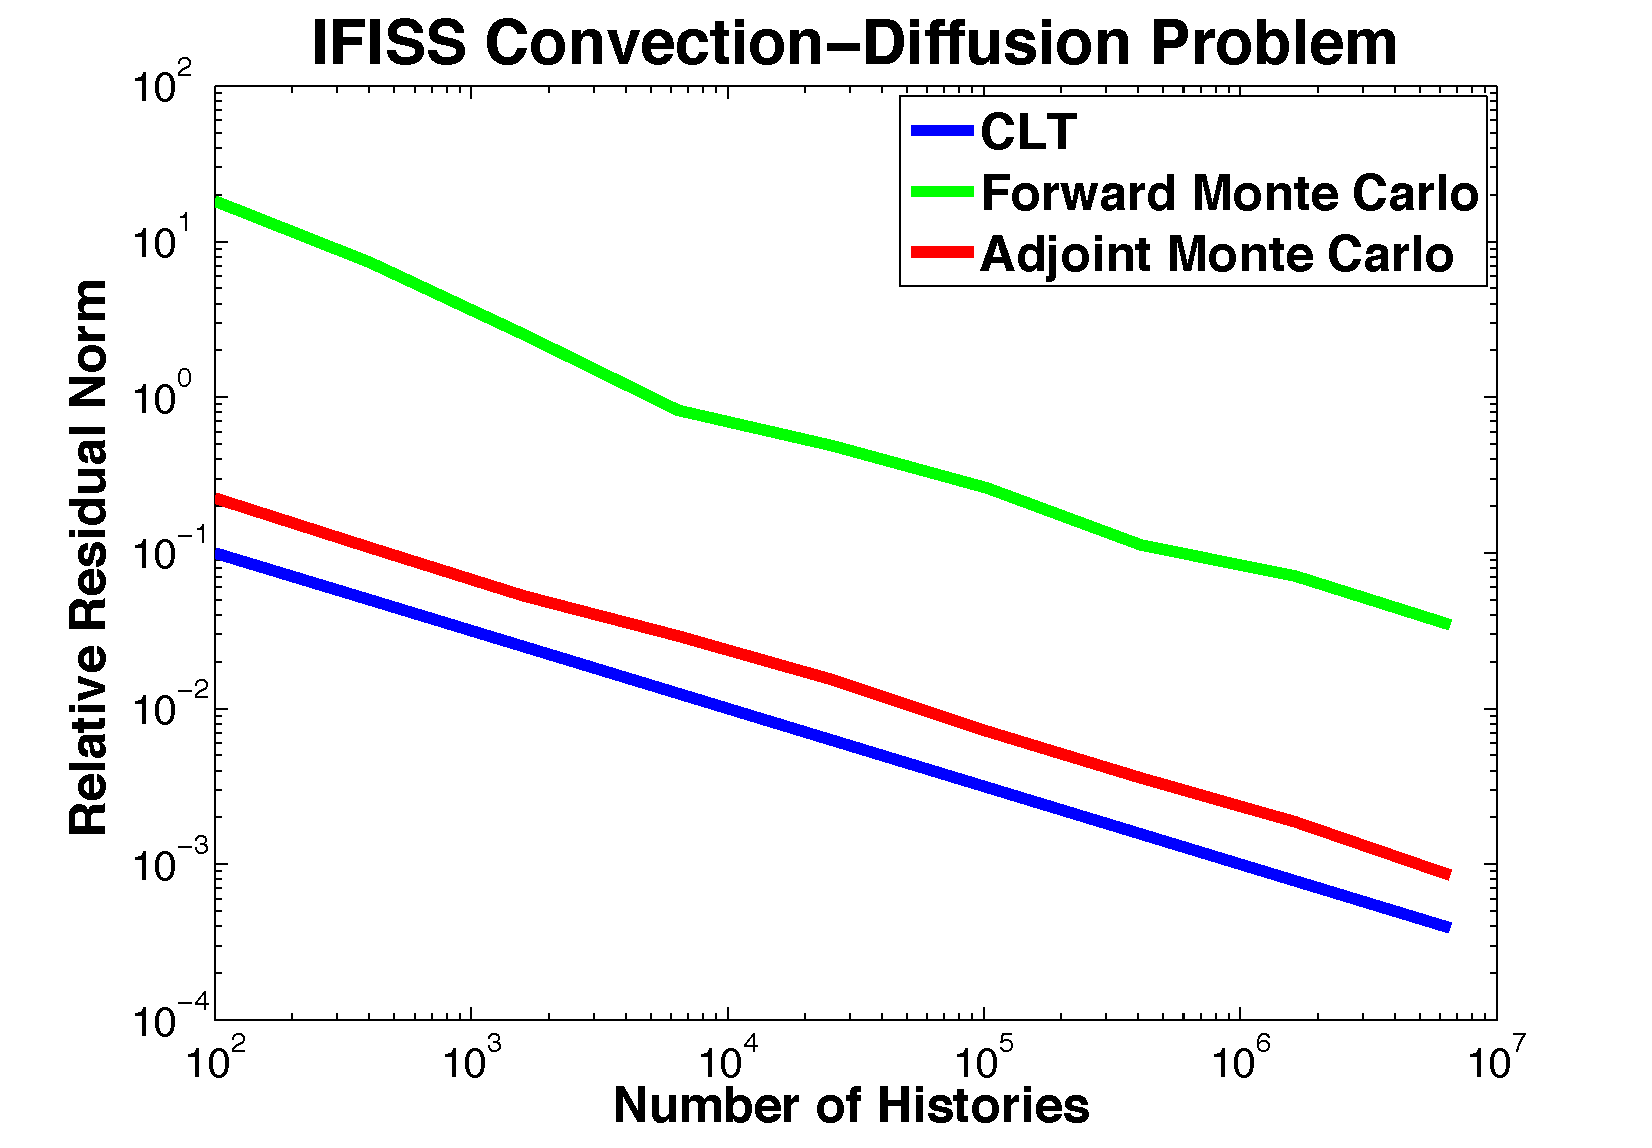
\includegraphics[width=1.75in]{../NCState_seminar_2014/Ifiss_ConvDiff}
    \end{figure}
  \item There is a potentially restrictive limit on the spectral properties of
    $\mathbf{H}$
    \begin{equation*}
      \rho(\mathbf{H}) < 1\:, \rho(\hat{\mathbf{H}}) < 1\:, \hat{H}_{ij} =
      \frac{H_{ij}^2}{P_{ij}}
    \end{equation*}
  \end{itemize}
\end{frame}

%%---------------------------------------------------------------------------%%

\begin{frame}{Monte Carlo Synthetic Acceleration}
  \begin{itemize}
  \item Address issue of convergence constrained by CLF
    \vfill
  \item Can be abstracted as a general linear solver
    \vfill
  \item Combine with Richardson iteration as a ``smoother'' in between
    Monte Carlo steps:
    \begin{align*}
      \mathbf{r}^k &= \mathbf{b} - \mathbf{Ax}^k \\
      \mathbf{x}^{k+1/2} &= \mathbf{x}^k + \mathbf{r}^k \\
      \mathbf{r}^{k+1/2} &= \mathbf{b} - \mathbf{Ax}^{k+1/2} \\
      \hat{\mathbf{A}} \mathbf{\delta} &= \mathbf{r}^{k+1/2} \\
      \mathbf{x}^{k+1} &= \mathbf{x}^{k+1/2} + \delta
    \end{align*}
  \item We still must address issue of convergence constraint by spectral radius
  \end{itemize}
\end{frame}

%%---------------------------------------------------------------------------%%

\begin{frame}{Monte Carlo as Approximate Polynomial Preconditioning}
  \begin{itemize}
    \item Using history length cutoff, Monte Carlo process is approximating
      a fixed length Neumann series polynomial
      \[
      x_i = \sum_{k=0}^{\infty}\sum_{i_1}^{N}\sum_{i_2}^{N}\ldots
      \sum_{i_k}^{N}h_{i,i_1}h_{i_1,i_2}\ldots h_{i_{k-1},i_k}b_{i_k}
      \]
    \vfill
    \item As number of histories grows, iteration count becomes identical to
      using ``true'' polynomial
    \vfill
    \item Why limit ourselves to the Neumann series polynomial?
      \begin{itemize}
        \item Chebyshev or GMRES polynomials are viable alternatives
      \end{itemize}
  \end{itemize}
\end{frame}

%%---------------------------------------------------------------------------%%

\begin{frame}{Neumann Series Polynomial}
  \begin{table}
    \caption{Adjoint MCSA with Neumann Polynomial, $1000 \times 1000$ Shifted Laplacian Matrix.
      Values are MCSA iteration counts (timing in milliseconds)
      \label{tab:lap_adjoint_neumann}}
    \centering
    \begin{tabular}{cccc}
      \toprule
      Histories per & \multicolumn{3}{c}{Polynomial Order} \\
      \cmidrule(lr){2-4}
      Iteration & 2 & 4 & 6 \\
      \midrule
      250 &  775(100) & 651(96) & 664(110) \\
      500 &  725(122) & 502(104) & 394(95) \\
      1000 & 707(174) & 482(179) & 366(144) \\
      2000 & 703(280) & 471(259) & 356(251) \\
      4000 & 698(494) & 467(497) & 350(458) \\
      8000 & 697(923) & 464(905) & 350(873) \\
      16000 & 695(1796) & 462(1768) & 347(1711) \\
      \bottomrule
    \end{tabular}
  \end{table}
\end{frame}

%%---------------------------------------------------------------------------%%

\begin{frame}{Chebyshev Polynomial}
  \begin{table}
    \caption{Adjoint MCSA with Chebyshev Polynomial, $1000 \times 1000$ Shifted Laplacian Matrix.
      Values are MCSA iteration counts (timing in milliseconds)
      \label{tab:lap_adjoint_cheby}}
    \centering
    \begin{tabular}{cccc}
      \toprule
      Histories per & \multicolumn{3}{c}{Polynomial Order} \\
      \cmidrule(lr){2-4}
      Iteration & 1 & 2 & 3 \\
      \midrule
      250 & - & - & - \\
      500 & - & - & - \\
      1000 & - & - & - \\
      2000 & - & 328(134) & - \\
      4000 & - & 296(210) & - \\
      8000 & - & 288(380) & 262(423) \\
      16000 & 1132(1866) & 283(721) & 175(550) \\
      \bottomrule
    \end{tabular}
  \end{table}
\end{frame}

%%---------------------------------------------------------------------------%%

\begin{frame}{Polynomial Methods -- Summary}
  \begin{itemize}
    \item Using history length cutoff rather than weight cutoff can lead to
      large reductions in iteration counts
      \vfill
    \item A good approximation to a few terms in the Neumann series
      performs better than a statistically noisy approximation to
      full series
      \vfill
    \item Significant reduction in iteration counts are possible using
      alternate polynomials, but partially offset by increase in number
      of histories required
      \begin{itemize}
        \item May be very beneficial from resiliency and parallel efficiency
          standpoints
        \item Will be re-evaluated in future efforts
      \end{itemize}
  \end{itemize}
\end{frame}

%%---------------------------------------------------------------------------%%

\begin{frame}{Preconditioning}
  \begin{itemize}
    \item Preconditioning needed to address convergence constraints due to
      spectral radius conditions
    \item Preconditioning for Monte Carlo introduces nonstandard considerations
      \begin{itemize}
      \item Elements of preconditioned matrix must be explicitly available,
        sparsity in $\mathbf{A}$, $\mathbf{M}$, does not imply sparsity in
        $\mathbf{M^{-1}A}$
        \item Goal of preconditioning is to reduce $\rho(\hat{\mathbf{H}})$,
          may not follow ``standard'' trends
      \end{itemize}
  \end{itemize}
  \vfill

  \begin{table}[!h]
  \centering
  \begin{tabular}{|c|c|c|c|}
  \hline
  \textbf{Block size} & \textbf{$\frac{nnz(H)}{nnz(A)}$}& $\rho(H)$
  &$\rho(\hat{H})$\\
  \hline
   3 & 1.4352 & $0.9804$ & $0.9531$\\
  \hline
   9 & 3.0220 & $0.9790$ & $0.9674$\\
  \hline
   33 & 9.8164 & $0.9783$  & $0.9774$\\
  \hline
  \end{tabular}
  \caption{$\rho(H)$ and $\rho(\hat{H})$ for advection--diffusion
  matrix with block diagonal preconditioning.}
  \label{tab:ifiss_block}
  \end{table}
\end{frame}

%%---------------------------------------------------------------------------%%

\begin{frame}{Preconditioning}
  \begin{itemize}
    \item Several options have been analyzed
      \begin{itemize}
        \item (Block) diagonal preconditioners, suitable for (block)
          diagonally dominant systems
        \item ILU-style preconditioners are possible, but require additional
          filtering to maintain sparsity in preconditioned system
        \item Approximate inverse preconditioning is attractive, forming
          preconditioned matrix only requires sparse matrix-matrix product
      \end{itemize}
  \end{itemize}

  \begin{table}[!h]
  \centering
  \begin{tabular}{|c|c|c|c|}
  \hline
  \textbf{Drop tolerance} & \textbf{$\frac{nnz(H)}{nnz(A)}$}& $\rho(H)$
  &$\rho(\hat{H})$\\
  \hline
   0.05 & 8.2797 & $0.9610$ & $1.0231$\\
  \hline
   0.01 & 33.1390 & $0.8668$ & $0.8279$\\
  \hline
  \end{tabular}
  \caption{$\rho(H)$ and $\rho(\hat{H})$ for 2D
  Laplacian with AINV preconditioning.}
  \label{tab:lap2d_ainv}
  \end{table}
\end{frame}

%%---------------------------------------------------------------------------%%

\begin{frame}{Domain Decomposed Monte Carlo}

  \begin{columns}
    \begin{column}{0.5\textwidth}
      \begin{itemize}
        \setlength{\itemsep}{-0.4\baselineskip}
      \item Each parallel process owns a piece of the domain (linear
        system)
        \bigskip
      \item Random walks must be transported between adjacent domains
        through parallel communication
        \bigskip
      \item Domain decomposition determined by the input system
        \bigskip
      \item Load balancing not yet addressed
        \bigskip
      \item Uses modified version of the Milagro algorithm (LANL)
      \end{itemize}
    \end{column}

    \begin{column}{0.5\textwidth}
      \begin{figure}[htpb!]
        \begin{center}
          \scalebox{0.75}{ \input{ddnu_example.pdftex_t} }
        \end{center}
        \caption{\small Domain decomposition example illustrating
          how domain-to-domain transport creates communication costs.}
      \end{figure}
    \end{column}
  \end{columns}

\end{frame}

%%---------------------------------------------------------------------------%%

\begin{frame}{Parallel Test - Simplified $P_N$ ($SP_N$) Assembly Problem}
\small
\begin{columns}

    \begin{column}{0.55\textwidth}

      \vspace{-0.2in}
      \begin{figure}
        \centering
        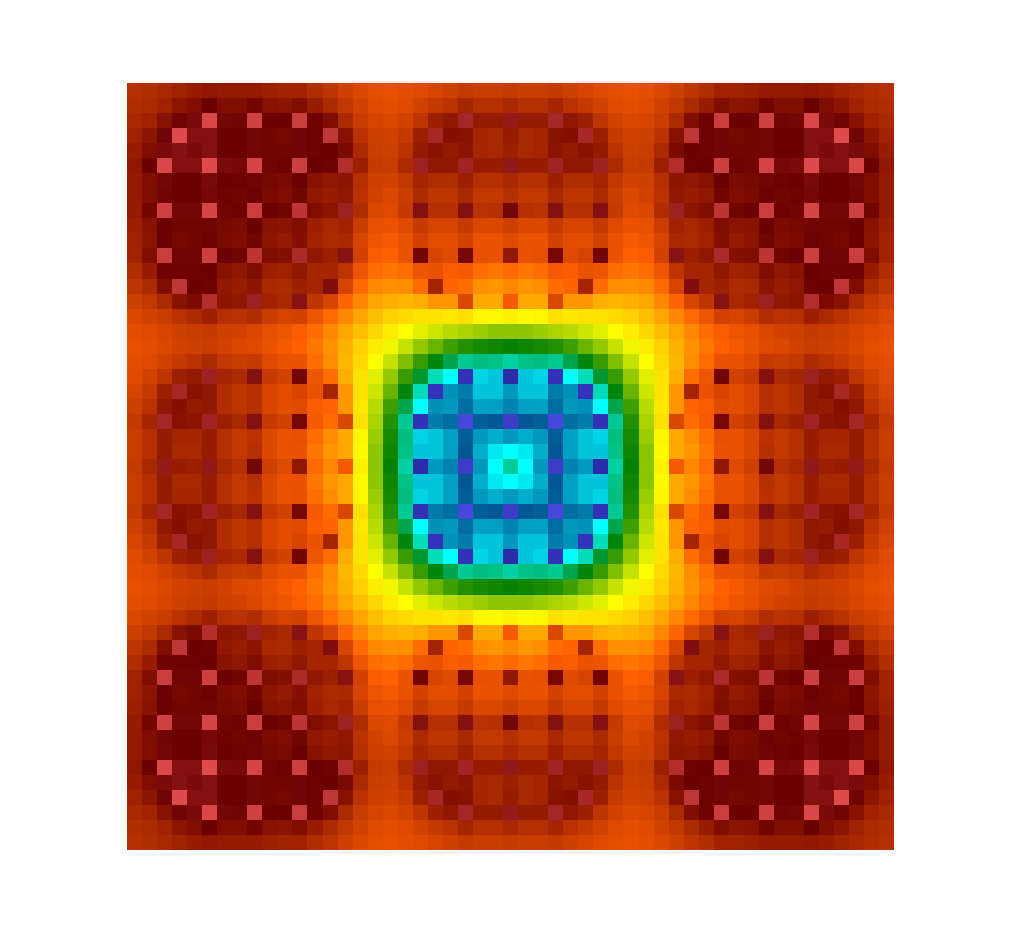
\includegraphics[width=2.0in]{../siam_cse_2015/presentation/prob4}
        \vspace{-0.2in}
        \caption{$SP_N$ solution example}
      \end{figure}

      \vspace{-0.1in}

      The ($SP_N$) equations are an approximation to the Boltzmann neutron
      transport equation used to simulate nuclear reactors

      \vspace{-0.2in}

      \[
        \small
        -\nabla \cdot \mathbb{D}_n \nabla \mathbb{U}_n + \sum_{m=1}^4
        \mathbb{A}_{nm} \mathbb{U}_m = \frac{1}{k} \sum_{m=1}^4
        \mathbb{F}_{nm} \mathbb{U}_m
      \]

    \end{column}

    \begin{column}{0.45\textwidth}
      Scaling problem -- $1 \times 1$ to $17 \times 17$ array of fuel
      assemblies with 289 pins each resolved by a $2 \times 2$ spatial mesh
      and 200 axial zones

      \vfill

      \begin{itemize}
      \item 7 energy groups, 1 angular moment, 1.6M to 273.5M degrees of
        freedom
      \item 64 to 10,800 computational cores via domain decomposition
      \item We are usually interested in solving generalized eigenvalue
        problem - we use the operator from these problems to test the kernel
        scaling
      \end{itemize}
    \end{column}

  \end{columns}

\end{frame}

%%---------------------------------------------------------------------------%%

\begin{frame}{Domain Decomposition Scaling}

  \vspace{-0.2in}

  \begin{table}[htb!]
    \tiny
    \begin{center}
      \begin{tabular}{rrrrrrr}
        \toprule
        \multicolumn{1}{r}{Cores} &
        \multicolumn{1}{r}{DOFs} &
        \multicolumn{1}{r}{DOFs/Core} &
        \multicolumn{1}{r}{Time Min (s)} &
        \multicolumn{1}{r}{Time Max (s)} &
        \multicolumn{1}{r}{Time Ave (s)} &
        \multicolumn{1}{r}{Efficiency}
        \\ \midrule
        %%
        256 & 273\,509\,600 & 1\,068\,397 & 515.51 & 515.52 & 515.52 & 1.00 \\
        1\,024 & 273\,509\,600 & 267\,099 & 122.76 & 122.77 & 122.76 & 1.05 \\ %CACHE
        4\,096 & 273\,509\,600 & 66\,775 & 27.96 & 27.97 & 27.96 & 1.15 \\
        7\,744 & 273\,509\,600 & 35\,319 & 17.72 & 17.72 & 17.72 & 0.96 \\
        10\,816 & 273\,509\,600 & 25\,288 & 13.72 & 13.72 & 13.72 & 0.89 \\
        %%
        \bottomrule
      \end{tabular}
    \end{center}
    \vspace{-0.07in}
    \caption{\small Strong Scaling}
  \end{table}

  \vspace{-0.4in}

  \begin{table}[htb!]
    \tiny
    \begin{center}
      \begin{tabular}{rrrrrrr}
        \toprule
        \multicolumn{1}{r}{Cores} &
        \multicolumn{1}{r}{DOFs} &
        \multicolumn{1}{r}{DOFs/Core} &
        \multicolumn{1}{r}{Time Min (s)} &
        \multicolumn{1}{r}{Time Max (s)} &
        \multicolumn{1}{r}{Time Ave (s)} &
        \multicolumn{1}{r}{Efficiency}
        \\ \midrule
        %%
        64 & 1\,618\,400 & 25\,288 & 12.65 & 12.65 & 12.65 & 1.00 \\
        256 & 6\,473\,600 & 25\,288 & 12.86 & 12.86 & 12.86 & 0.98 \\
        1\,024 & 25\,894\,400 & 25\,288 & 14.59 & 14.59 & 14.59 & 0.87 \\
        4\,096 & 103\,577\,600 & 25\,288 & 14.25 & 14.25 & 14.25 & 0.89 \\
        7\,744 & 195\,826\,400 & 25\,288 & 14.75 & 14.78 & 14.75 & 0.86 \\
        10\,816 & 273\,509\,600 & 25\,288 & 13.72 & 13.72 & 13.72 & 0.92 \\
        %
        \bottomrule
      \end{tabular}
    \end{center}
        \vspace{-0.07in}
    \caption{\small Weak Scaling}
  \end{table}

  \vspace{-0.25in}

  \begin{itemize}
    \small
  \item Titan Cray XK7 was used with no GPUs - used Eos parameters
  \item Results are consistent with transport literature
  \item History length of 15 and 3 histories per DOF
  \item Consider these effective operator apply times of 15 realizations of
    $\ve{H}$
  \item MC dominates run times in solver applications
  \end{itemize}

\end{frame}


%%---------------------------------------------------------------------------%%

\begin{frame}{Replication}

  \vspace{-0.1in}

  Different batches of Monte Carlo samples can be combined in summation via
  superposition if they have different random number streams.  Consider each
  of these batches independent \textit{subsets} of a Monte Carlo operator
  where now the operator can be formed as a general additive decomposition of
  $N_S$ subsets:

  \[
  \mathbf{M_{MC}} = \frac{1}{N_S}\sum_{n=1}^{N_s}{\mathbf{M_n}}
  \]

  We replicate the linear problem and form each subset on a different group of
  parallel processes. Applying the subsets to a vector requires an AllReduce
  to form the sum. Each subset is domain decomposed.
  \vfill
  This provides a mechanism to support \textit{resiliency}; the replicated
  component provides {\bf useful} work, not just redundancy

\end{frame}

%%---------------------------------------------------------------------------%%

\begin{frame}{Replication Scaling}

  \begin{table}[htb!]
    \tiny
    \begin{center}
      \begin{tabular}{rrrrrrr}
        \toprule
        \multicolumn{1}{r}{Subsets} &
        \multicolumn{1}{r}{Cores} &
        \multicolumn{1}{r}{DOFs} &
        \multicolumn{1}{r}{Time Min (s)} &
        \multicolumn{1}{r}{Time Max (s)} &
        \multicolumn{1}{r}{Time Ave (s)} &
        \multicolumn{1}{r}{Efficiency}
        \\ \midrule
        %%
        1 & 256 & 6\,473\,600 & 12.65 & 12.65 & 12.65 & 1.00 \\
        2 & 512 & 6\,473\,600 & 6.62 & 6.80 & 6.72 & 0.93 \\
        3 & 768 & 6\,473\,600 & 4.50 & 4.73 & 4.66 & 0.89 \\
        4 & 1\,024 & 6\,473\,600 & 3.62 & 3.81 & 3.71 & 0.83 \\
        %
        \bottomrule
      \end{tabular}
    \end{center}
    \caption{\small Fixed algorithmic scaling}
  \end{table}

  \vfill

  \begin{itemize}
    \small
  \item Timings are Monte Carlo time plus AllReduce time
  \item 256 cores per subset with domain decomposition
  \item $1/N_S$ samples per subset gives flat algorithmic performance
  \item Two performance issues
    \begin{itemize}
    \item Dividing up samples creates work starvation
    \item AllReduce buffer size is constant regardless of work starvation
    \end{itemize}
  \item Research is needed for a more performant subset combination
  \end{itemize}

\end{frame}

%%---------------------------------------------------------------------------%%

\begin{frame}{GPU Optimization}

  We have implemented a version of MCSA that uses GPUs to perform the MC
  linear solve.

  Distributed parallelism is enabled through an additive Schwartz method, all
  MC solves
  \begin{itemize}
  \item All MC random walks are local
  \item No inter-domain communication of histories
  \end{itemize}

  \begin{table}[h]
    \begin{center}
      \caption{2D parabolic problem with AINV preconditioning.}
      \begin{tabular}{|c|c|c|c|}\hline
        Node & Iterations & Time (sec) & Relative Residual \\\hline
        CPU & 6 & 992.23 & $1.23\times 10^{-7}$ \\\hline
        GPU & 6 & 29.83 & $1.53\times 10^{-7}$ \\\hline
      \end{tabular}
    \end{center}
  \end{table}

\end{frame}

%%---------------------------------------------------------------------------%%
\subsection{Research Requirements}
%%---------------------------------------------------------------------------%%

\begin{frame}{Continued Research is Necessary}

  The following important questions need to be answered before MC methods can
  be applied to linear systems as a ``standard'' solver:

  \begin{itemize}
  \item Automatically determine history termination criteria
    \begin{itemize}
    \item We have investigated adaptive schemes based on variance
    \item However, variance is not directly correlated with error
    \end{itemize}
  \item Identify classes of matrices and preconditioners that satisfy
    convergence constraints
    \begin{itemize}
    \item This has been done for SDD and GDD
    \end{itemize}
  \item Demonstrate resiliency to hard MPI errors through replicated domain
    parallelism
  \item Further investigate non-linear, time-dependent problems
    \begin{itemize}
    \item This was part of the original proposal
    \item Non-linear, sub-cycle time-stepping can result in strongly diagonally
      dominant problems for which MCSA has been shown to be effective
    \end{itemize}
  \end{itemize}
\end{frame}

%%---------------------------------------------------------------------------%%
\subsection{Software}
%%---------------------------------------------------------------------------%%

\begin{frame}{MCSA Implementations}


  {\bf MCLS} (\underline{github.com/sslattery/MCLS})
  \begin{itemize}
  \item Massively parallel (MPI) implementation of domain decomposed MCSA
    algorithm
  \item Implemented in Trilinos framework and callable through Trilinos'
    abstract numerical algorithms (Thyra, Stratimikos) interface
  \item Works with any Tpetra row matrix
  \end{itemize}
  \vfill
  {\bf Alea} (\underline{github.com/ORNL-CEES/Profugus})
  \begin{itemize}
  \item GPU-accelerated on-node MC solve
  \item Domain-local MC solves implemented for distributed systems as an
    additive Schwartz method
  \end{itemize}
  \vfill
  All software is BSD open source.
  \vfill
  Uses TriBITS (Trilinos) open source build system
  \vfill
  Both software packages contain a complete suite of unit-tests integrated
  through GoogleTest (Alea) or TeuchosTest (MCLS)
\end{frame}

%%---------------------------------------------------------------------------%%

\begin{frame}{Publications and Presentations}

  \underline{Publications}
  \begin{itemize}
  \item M. Benzi, T.M. Evans, S.P. Hamilton, M.L. Pasini, and
    S.R. Slattery. Analysis of Monte Carlo Accelerated Iterative Methods for
    Sparse Linear Systems. \textit{in preparation}, 2016.
  \item S.R. Slattery, T.M. Evans, P.P.H. Wilson. A Spectral Analysis of the
    Domain Decomposed Monte Carlo Method for Linear Systems. \textit{Nuclear
      Engineering Design},  {\bf 295}, 632--638, 2015.
  \item T.M. Evans, S.W. Mosher, S.R. Slattery, and S.P. Hamilton. A Monte Carlo
    Synthetic Acceleration Method for Solving the Thermal Radiation Diffusion
    Equation. \textit{J. Comp. Phys.}, {\bf 258}, 338--358, 2014.
  \end{itemize}

\end{frame}

%%---------------------------------------------------------------------------%%

\begin{frame}{Publications and Presentations}

  \underline{Presentations}
  \begin{itemize}
    \footnotesize
    \setlength{\itemsep}{-0.1\baselineskip}
  \item Monte Carlo Synthetic Acceleration Methods for Sparse Linear Systems
    (M.L. Pasini, M. Benzi, T. Evans, S. Hamilton, S. Slattery), \textit{SIAM
      ALA}, October 30, 2015.
  \item Parallel Algorithms for the Monte Carlo Synthetic Acceleration Linear
    Solver Method (S. Slattery, T. Evans, S. Hamilton), \textit{SIAM CSE},
    Salt Lake City, 2015.
  \item Iterative Performance of Monte Carlo Linear Solver Methods
    (M.L. Pasini), \textit{SIAM CSE}, Salt Lake City, 2015.
  \item A multilevel Monte Carlo method for linear systems (S. Slattery,
    T. Evans, S. Hamilton), \textit{Copper Mountain Conference on Iterative
      Solvers}, Copper MT, CO, 2014.
  \item Monte Carlo Synthetic Acceleration as approximate polynomial
    preconditioning (S. Hamilton, T. Evans, S. Slattery), \textit{Copper
      Mountain Conference on Iterative Solvers}, Copper MT, CO, 2014.
  \item Monte Carlo Linear Solvers (S. Slattery, T. Evans, S. Hamilton),
    \textit{NC State Seminar}, Nov. 4, 2014.
  \item Monte Carlo Linear Solvers (S. Hamilton, T. Evans, S. Slattery),
    \textit{Emory Mathematics Dept. Seminar}, Sept. 19, 2014.
  \item Monte Carlo Methods for Linear Systems (T. Evans), \textit{MIT Nuclear
      Engineering Dept Seminar Series}, Sept. 30, 2014.
  \end{itemize}

\end{frame}

%%---------------------------------------------------------------------------%%
\section{Transition and Roadmap}
%%---------------------------------------------------------------------------%%
\subsection{ECP Application Requirements}
%%---------------------------------------------------------------------------%%

\begin{frame}{Connection to ECP Requirements}

  \begin{itemize}

  \item Inter-Operability
    \begin{itemize}
    \item MCLS built using Trilinos solver API
    \item Utilizes Hypre/ParaSAILS for AINV preconditioning
    \item Enables testing of MC solver algorithms in a wide variety of
      applications, ie. anyone who uses Trilinos
    \end{itemize}

  \item Scalability
    \begin{itemize}
    \item Multilevel inter-node domain decomposition methods show excellent
      scalability
    \item GPU-enabled on-node MC kernel yields measures speedups of 30 -
      50$\times$
    \end{itemize}

  \item Resiliency
    \begin{itemize}
    \item Replicated subsets enable useful work to occur at the same time as
      providing redundancy
    \item Yields protection against hard errors
    \end{itemize}
  \end{itemize}

\end{frame}

%%---------------------------------------------------------------------------%%

\begin{frame}{Inter-Operatibility Example}

  Using the MCLS interface to Trilinos, it is straightforward to implement
  MCSA in other applications
  \vfill
  We implemented MCSA in the production CFD code, Drekar (SNL) using a
  Newton-MCSA algorithm:
  \begin{algorithm}[H]
    \footnotesize
    \begin{algorithmic}[1]
      \STATE $k := 0$
      \WHILE{$||\ve{F}(\ve{u}^{k})|| > \epsilon
        ||\ve{F}(\ve{u}^{0})||$}
      \STATE $\ve{J}(\ve{u}^{k}) \leftarrow AD(\ve{F}(\ve{u}^k))$
      \COMMENT{Automatic differentiation - Panzer}
      \STATE $\ve{J}(\ve{u}^k) \delta \ve{u}^k = -\ve{F}(\ve{u}^{k})$
      \COMMENT{Solve for the Newton correction with MCSA}
      \STATE $\ve{u}^{k+1} \leftarrow \ve{u}^k + \delta \ve{u}^k$
      \STATE $k \leftarrow k+1$
      \ENDWHILE
    \end{algorithmic}
    \caption{FANM}
  \end{algorithm}
  \vfill
  Because MCLS was built with Trilinos abstract numerical algorithms this
  integration was straightforward and we can test MCLS in a whole new problem
  space
  \vfill
  We are also able to utilize all of Trilinos' preconditioners

\end{frame}

%%---------------------------------------------------------------------------%%

\begin{frame}{Thermal Convection Cavity Results}

  \begin{columns}
    \begin{column}{0.6\textwidth}

      \small{
        \begin{table}[h!]
          \begin{center}
            \begin{tabular}{lccc}\hline\hline
              \multicolumn{1}{l}{Benchmark}&
              \multicolumn{1}{c}{NK}&
              \multicolumn{1}{c}{FANM}&
              \multicolumn{1}{c}{NR}\\
              \hline
              Ra=\sn{1}{3} & 5 & 5 & 5\\
              Ra=\sn{1}{4} & 7 & 7 & 7\\
              Ra=\sn{1}{5} & 9 & 10 & 9\\
              Ra=\sn{1}{6} & 11 & 11 & 11\\
              %%
              \hline\hline
            \end{tabular}`
          \end{center}
          \caption{Nonlinear iterations.}
        \end{table}

        \begin{table}[h!]
          \begin{center}
            \begin{tabular}{lccc}\hline\hline
              \multicolumn{1}{l}{Benchmark}&
              \multicolumn{1}{c}{GMRES}&
              \multicolumn{1}{c}{MCSA}&
              \multicolumn{1}{c}{Richardson}\\
              \hline
              Ra=\sn{1}{3} & 32 & 18 & 38\\
              Ra=\sn{1}{4} & 23 & 17 & 34\\
              Ra=\sn{1}{5} & 25 & 20 & 34\\
              Ra=\sn{1}{6} & 39 & 25 & 48\\
              %%
              \hline\hline
            \end{tabular}
          \end{center}
          \caption{Total linear solver iterations.}
        \end{table}
      }

    \end{column}

    \begin{column}{0.4\textwidth}

      \small{
        \begin{itemize}
        \item Weaker preconditioning at Ra=\sn{1}{5} case
          \medskip
        \item Constant forcing term for Ra=\sn{1}{6} case
        \end{itemize}
      }

      \bigskip

      \tiny{
        \begin{table}[h!]
          \begin{center}
            \begin{tabular}{lc}\hline\hline
              \multicolumn{1}{l}{Benchmark}&
              \multicolumn{1}{c}{NK Speedup}\\
              \hline
              Ra=\sn{1}{3} & 338 \\
              Ra=\sn{1}{4} & 336 \\
              Ra=\sn{1}{5} & 346 \\
              Ra=\sn{1}{6} & 465 \\
              \hline\hline
            \end{tabular}
          \end{center}
          \caption{Newton-Krylov speedup over FANM.}
        \end{table}
      }

    \end{column}
  \end{columns}

\end{frame}

%%---------------------------------------------------------------------------%%

\begin{frame}{ECP Coordinated Reasearch}

  \underline{\bf Goal}: Extend the general algorithmic MC exascale methods
  w.r.t. scalability and resiliency into a broader application space

  MC methods are used in many DOE application areas:
  \begin{itemize}
    \setlength{\itemsep}{-0.2\baselineskip}
  \item high-energy density physics
  \item astrophysics
  \item nuclear engineering
  \item particle accelerators and neutron spallation source
  \item quantum chemistry
  \item visualization
  \item fluid dynamics
  \item combustion
  \item computational biology
  \end{itemize}

  Much of the algorithmic research performed in MCREX is directly applicable
  to the use of MC methods in these other application areas

\end{frame}

%%---------------------------------------------------------------------------%%

\begin{frame}{ECP R\&D I: Time-dependent Problems}

  Investigate use in time-dependent applications, e.g. non-linear radiation
  hydrodynamics for high-energy density physics applications:
  \begin{itemize}
  \item Used as inner linear solver in a non-linear (Newton) iteration
  \item Time-dependent applications generally have strong diagonal-dominance
    that makes MCSA competitive with Krylov methods
  \item MCSA has resiliency and parallel efficiency benefits over subspace
    methods
  \end{itemize}

\end{frame}

%%---------------------------------------------------------------------------%%

\begin{frame}{ECP R\&D II: Monte Carlo Particle Transport}

  MC particle transport has applications in many areas across the DOE complex
  \begin{itemize}
    \setlength{\itemsep}{-0.2\baselineskip}
  \item high-energy density physics
  \item neutron spallation source
  \item nuclear engineering
  \item astrophysics
  \item combustion
  \end{itemize}

  \vfill

  There are significant challenges in porting random walk algorithms to modern
  heterogeneous computing devices
  \begin{enumerate}
  \item Random walks are dominated by branching statements $\rightarrow$
    thread divergence
  \item Runtime is often dominated by sampling and interpolating large fields
    of data (keeping the GPUs fed)
  \end{enumerate}

  \vfill

  Supporting research into the efficient parallelization and instrumentation
  of random walk algorithms for particle transport will benefit many
  applications in DOE

\end{frame}

%%---------------------------------------------------------------------------%%

\begin{frame}{ECP R\&D III: Particle Methods}

  Non-stochastic particle methods share a great deal of algorithmic features
  with stochastic particle methods
  \begin{itemize}
  \item Particles must be ordered and sorted efficiently
  \item Particles must be moved through a combinatorial and mesh-based
    geometries
  \item Data structures must be optimized for efficient vectorization (over
    32-thread warps on GPUs)
  \item Inter-node communication of particle data structures are required for
    domain decomposition parallel topologies
  \item Physical parameters must be mapped between particles and an underlying
    data representation (grid)
  \end{itemize}

  \vfill

  A supporting technolgies research effort on a generalized set of libraries
  for managing particle-based data structures on heterogeneous computing
  platforms will benefit many applications in DOE

\end{frame}

%%---------------------------------------------------------------------------%%

\begin{frame}{Building on ASCR Funding}

  \underline{\bf Trilinos}
  \begin{itemize}
  \item Provides abstract solver interface for MCLS
  \item Provides build system for Alea and MCLS
  \item Provides data structures and utilities for Alea and MCLS
  \end{itemize}

  \vfill

  \underline{\bf xSIM}
  \begin{itemize}
  \item Simulator to test for hard error detection and remediation
  \end{itemize}

\end{frame}

%%---------------------------------------------------------------------------%%

\begin{frame}{Building on ASCR Funding}

  \underline{\bf XPRESS}
  \begin{itemize}
  \item We are currently implementing a CUDA transport kernel with scheduling
    optimized by HPX as part of XPRESS
  \item We have already compared OpenMP versus HPX for on-node MC particle
    transport algorithms
  \end{itemize}

  \begin{figure}
    \centering
    \begin{tabular}{cc}
      \subfigure[time]{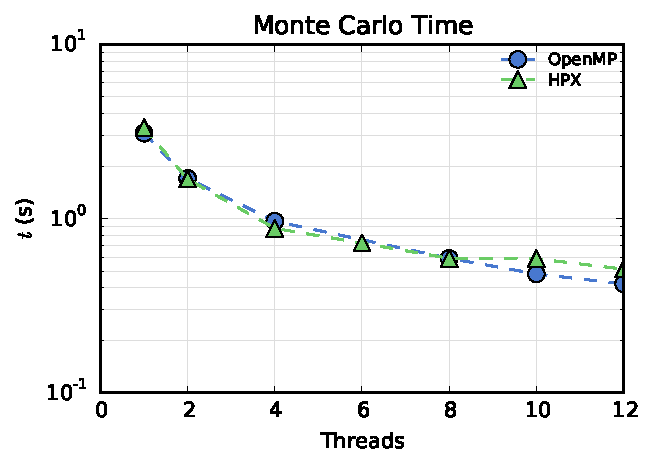
\includegraphics[width=2in]{time}}
      &
      \subfigure[efficiency]{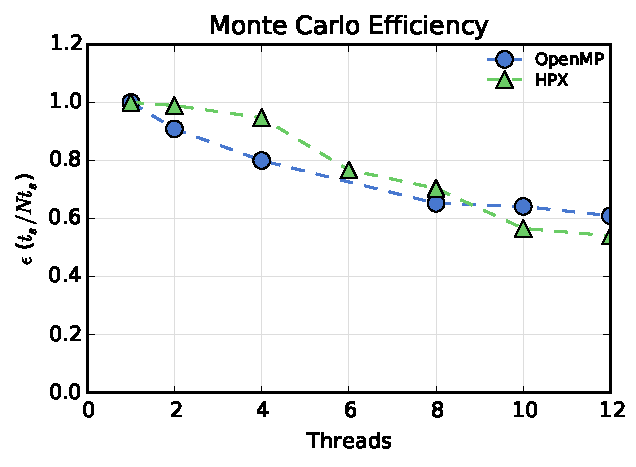
\includegraphics[width=2in]{tallies}}
    \end{tabular}
  \end{figure}

\end{frame}

%%---------------------------------------------------------------------------%%

\begin{frame}
\vfill
\centering
\huge Questions?
\vfill
\end{frame}

%%---------------------------------------------------------------------------%%
\section*{Extra Slides}
%%---------------------------------------------------------------------------%%

\begin{frame}{Preconditioned MCSA}
\vspace*{-0.2in}
  {
    \small
    \[
    \ve{r}^{k} = \ve{M}_L^{-1}(\ve{b}-\ve{A}\ve{M}_R^{-1}\ve{x}^{k})
    \]
    \[
    \ve{x}^{k+1/2} = \ve{x}^k + \ve{r}^k
    \]
    \[
    \ve{r}^{k+1/2} = \ve{M}_L^{-1}(\ve{b}-\ve{A}\ve{M}_R^{-1}\ve{x}^{k+1/2})
    \]
    \[
    \ve{M}_L^{-1}\ve{A}\ve{M}_R^{-1}\delta\ve{x}^{k+1/2} = \ve{r}^{k+1/2}
    \]
    \[
    \ve{x}^{k+1} = \ve{x}^{k+1/2} + \delta \ve{x}^{k+1/2}
    \]
  }
  \vspace*{-0.1in}
  \begin{itemize}
    \item Requires explicit construction of preconditioned matrix
      \begin{itemize}
        \item This has generally limited preconditioner selection to diagonal,
          block diagonal, sparse approximate inverse approaches
      \end{itemize}
    \vfill
    \item Sparsity in $\mathbf{A}$, $\mathbf{M}$, does not imply sparsity
      in $\mathbf{M^{-1}A}$
    \vfill
    \item Need to investigate preconditioning strategies that lead to sparse
      preconditioned systems
  \end{itemize}
\end{frame}

%%---------------------------------------------------------------------------%%

\begin{frame}{Asynchronous Monte Carlo Transport Kernel}

  \begin{columns}

    \begin{column}{0.5\textwidth}
      \vspace{-0.1in}
      \small
      \begin{itemize}
      \item General extension of the Milagro algorithm (LANL)
      \item Asynchronous nearest neighbor communication of histories
      \item System-tunable communication parameters of buffer size and check
        frequency (performance impact)
      \item Need an asynchronous strategy for exiting the transport loop
        without a collective (running sum)
      \end{itemize}

      \vspace{-0.15in}
      \begin{figure}[htpb!]
        \begin{center}
          \scalebox{0.4}{ \input{domain_to_domain.pdftex_t} }
        \end{center}
      \end{figure}

    \end{column}

    \begin{column}{0.5\textwidth}

      \vspace{-0.25in}
      \begin{figure}[htpb!]
        \begin{center}
          \scalebox{0.825}{ \input{transport_loop.pdftex_t} }
        \end{center}
      \end{figure}

    \end{column}

  \end{columns}

\end{frame}

%%---------------------------------------------------------------------------%%
\end{document}
%%---------------------------------------------------------------------------%%

%%---------------------------------------------------------------------------%%
%% end of pres.tex
%%---------------------------------------------------------------------------%%
